\documentclass[11pt]{article}
\usepackage[margin=0cm,nohead]{geometry}
\usepackage[active,tightpage]{preview}

\usepackage{tikz,amsmath,amssymb,bm,color,cancel}

%\usepackage{newtxtext}
%\usepackage{newtxmath}

\usetikzlibrary{shapes,arrows}
\usetikzlibrary{calc}
\usetikzlibrary{positioning}
\usetikzlibrary{decorations.pathreplacing}

\PreviewEnvironment{tikzpicture}
\setlength\PreviewBorder{-1mm}

\begin{document}

\begin{tikzpicture}

%%%%%%%%%%%%%%%%%%%%%%%%%%%%%%%%%%%%%%%%%%%%%%%%%%%%%%%%%%%%%% Macros

\newcommand{\bb}[2]{
	\!\!{\tt #1}
	\\[6pt]
	~{\large \color{blue} #2}
}
\newcommand{\bbb}[3]{
	\!\!{\tt #1}
	\\[6pt]
	~{\large \color{blue} #2}
	\\[6pt]
	~{#3}
}

\newcommand{\tr}{\mathsf{{\scriptscriptstyle T}}}
\newcommand{\ii}{\mathrm{i}}
\newcommand{\ee}{\operatorname{e}}
\newcommand{\dd}{\mathrm{d}}
\newcommand{\op}[1]{\operatorname{#1}}

\newcommand{\pL}{\mathsf{{\scriptscriptstyle L}}}
\newcommand{\pR}{\mathsf{{\scriptscriptstyle R}}}
\newcommand{\pC}{\mathsf{{\scriptscriptstyle C}}}

\newcommand{\bPsi}{\boldsymbol{\Psi}}
\newcommand{\bPhi}{\boldsymbol{\Phi}}

\newcommand{\suY}{\mathrm{\scriptscriptstyle Y}}
\newcommand{\suL}{\mathrm{\scriptscriptstyle L}}
\newcommand{\suC}{\mathrm{\scriptscriptstyle C}}

\newcommand{\dbar}[1]{\overline{#1}}
\newcommand{\sbar}[1]{\bar{#1}}
\newcommand{\anti}[1]{\bar{#1}}

\newcommand{\quantNo}[3]{\mathbf{#1},\mathbf{#2},#3}
 
%%%%%%%%%%%%%%%%%%%%%%%%%%%%%%%%%%%%%%%%%%%%%%%%%%%%%%%%%%%%%% Box styles

\tikzset{myRow/.style     ={draw,anchor=north west,rectangle}}
\tikzset{boxWhite/.style  ={draw,anchor=north west,rectangle, very thin, rounded corners=5pt, fill=white}}
\tikzset{boxGray/.style   ={draw,anchor=north west,rectangle, very thin, rounded corners=5pt, fill=gray!10}}
\tikzset{boxRed/.style    ={draw,anchor=north west,rectangle, very thin, rounded corners=5pt, fill=red!4}}
\tikzset{boxGreen/.style  ={draw,anchor=north west,rectangle, very thin, rounded corners=5pt, fill=green!2}}
\tikzset{boxYellow/.style ={draw,anchor=north west,rectangle, very thin, rounded corners=5pt, fill=yellow!5}}
\tikzset{boxBlue/.style   ={draw,anchor=north west,rectangle, very thin, rounded corners=5pt, fill=blue!2}}
\tikzset{boxCyan/.style   ={draw,anchor=north west,rectangle, very thin, rounded corners=5pt, fill=cyan!2}}
\tikzset{colorLagr/.style ={fill=magenta!8}}

%%%%%%%%%%%%%%%%%%%%%%%%%%%%%%%%%%%%%%%%%%%%%%%%%%%%%%%%%%%%%% R/C styles

\tikzset{R10/.style={minimum height=10mm}}
\tikzset{R15/.style={minimum height=15mm}}
\tikzset{R20/.style={minimum height=20mm}}
\tikzset{R25/.style={minimum height=25mm}}
\tikzset{R30/.style={minimum height=30mm}}
\tikzset{C10/.style={minimum width=10mm}}
\tikzset{C15/.style={minimum width=15mm}}
\tikzset{C20/.style={minimum width=20mm, text width=17mm}}
\tikzset{C25/.style={minimum width=25mm, text width=22mm}}
\tikzset{C30/.style={minimum width=30mm, text width=27mm}}
\tikzset{C35/.style={minimum width=35mm, text width=32mm}}
\tikzset{C40/.style={minimum width=40mm, text width=37mm}}
\tikzset{C45/.style={minimum width=45mm, text width=42mm}}
\tikzset{C50/.style={minimum width=50mm, text width=47mm}}
\tikzset{C55/.style={minimum width=55mm, text width=52mm}}
\tikzset{C60/.style={minimum width=60mm, text width=57mm}}
\tikzset{C65/.style={minimum width=65mm, text width=62mm}}
\tikzset{C70/.style={minimum width=70mm, text width=67mm}}
\tikzset{C75/.style={minimum width=75mm, text width=72mm}}
\tikzset{C80/.style={minimum width=80mm, text width=77mm}}
\tikzset{C85/.style={minimum width=85mm, text width=82mm}}
\tikzset{C90/.style={minimum width=90mm, text width=87mm}}
\tikzset{C95/.style={minimum width=95mm, text width=92mm}}
\tikzset{C100/.style={minimum width=100mm, text width=97mm}}

%%%%%%%%%%%%%%%%%%%%%%%%%%%%%%%%%%%%%%%%%%%%%%%%%%%%%%%%%%%%%% Paper W/H

%\draw [yellow] (-0.5*\paperWidth,-0.5*\paperHeight) rectangle (0.5*\paperWidth,0.5*\paperHeight);
%\draw [red,dashed] (-0.5*\paperWidth,-0.5*\paperHeight) rectangle (0.5*\paperWidth,0.5*\paperHeight);
%\draw [blue!40] (-20.5,14.5) rectangle (20.5,-14.5);

\node at (-20.5,14.5) {}; \node at (20.5,-14.5) {};

%%%%%%%%%%%%%%%%%%%%%%%%%%%%%%%%%%%%%%%%%%%%%%%%%%%%%%%%%%%%%% SM-charges pdf

\node [anchor=north west] at (9.5,-0.75) {
	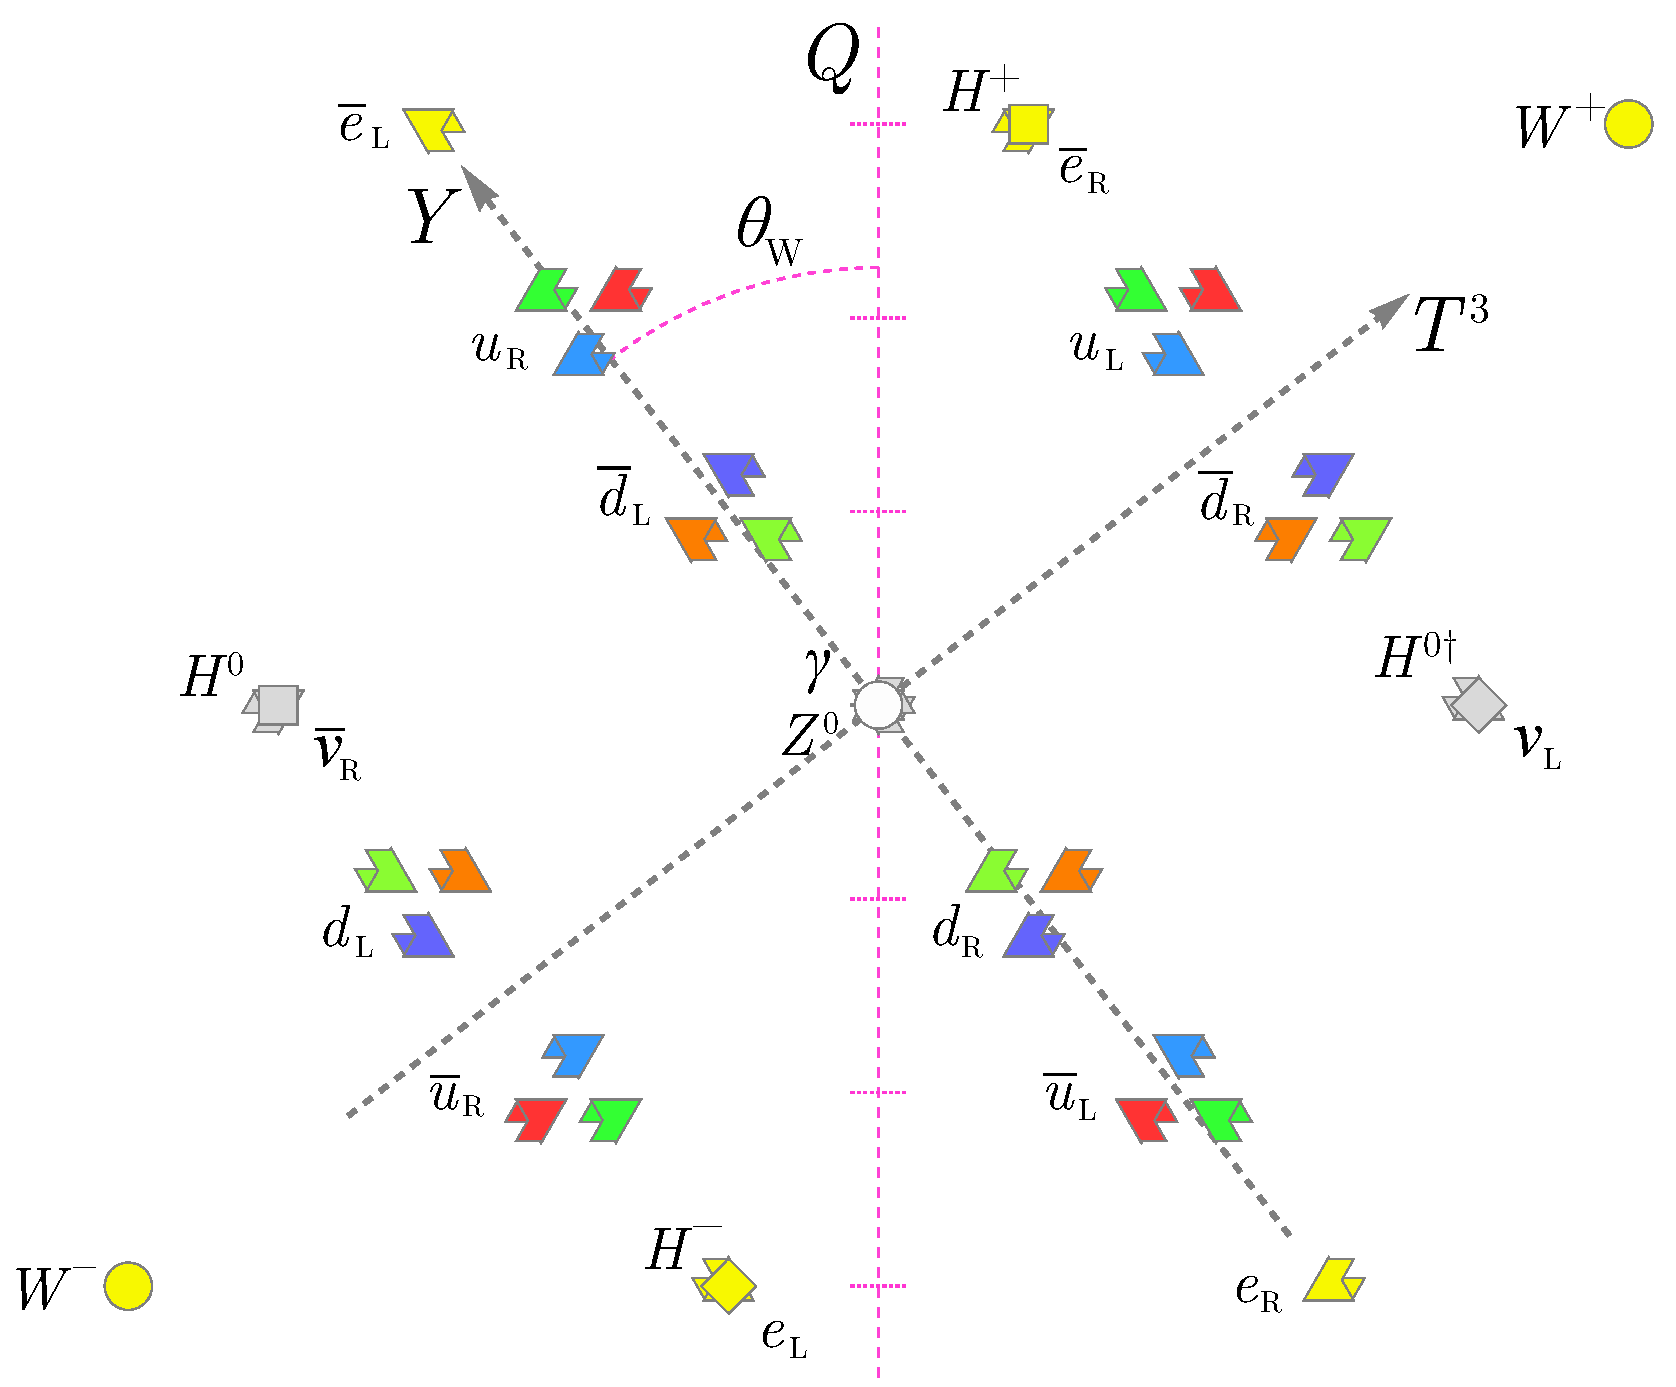
\includegraphics[width=110mm]{sw-charges.pdf}
};

\draw (11.4686,-5.5056) -- (9,-6.75);

\node [anchor=north west, C60] at (6.25,-6.75) { \footnotesize
	The neutral Higgs field which \\breaks the EW symmetry. \\
	($H^\pm, H^{0\dagger}$ are eaten by $W^\pm, Z^0$)
};

%%%%%%%%%%%%%%%%%%%%%%%%%%%%%%%%%%%%%%%%%%%%%%%%%%%%%%%%%%%%%% Title

\node [color=black] at (0,14.25) {
	\huge\sf The field content of the Standard Model (SM)
};

\node [anchor=north, color=black] at (0,13.9) {
	by M.B.Kocic ~--~ Version 1.04 (2016-01-21) ~--~ FK8017 HT15
};

\pdfinfo {
%	/CreationDate	(D:20160121124500)
	/Title			(The field content of the Standard Model (SM))
	/Author			(Mikica B Kocic)
	/Subject		(FK8017 HT15)
	/Keywords		(QFT SM)
	/Creator		(TeX-TikZ)
}

\node [boxGreen,anchor=north west,C85] at (12,14) {
	\textsf{ The SM Lagrangian $=$ Sum of the kinetic terms \\
	\quad $+$ the Higgs potential \\
	\quad $+$ the Yukawa interaction terms }
};

%%%%%%%%%%%%%%%%%%%%%%%%%%%%%%%%%%%%%%%%%%%%%%%%%%%%%%%%%%%%%% Vector bosons

\tikzset{myRow/.style={boxRed,R10}}

\node [myRow,C40,align=center] at (-20.5,13) {
	\textsf{\textbf{Vector bosons}}
};

\node [myRow,C40,align=center] at (-16.5,13) {
	Field
};

\node [myRow,C20,align=center] at (-12.5,13) {
	Adj.repr.
	%/ $\mathrm{Q.N^{\underline{o}}}$
};

\node [myRow,C45,align=center] at (-10.5,13) {
	Charge
};

\node [myRow,colorLagr,C35,align=center] at (-6,13) {
	Kinetic term % $(\mathcal{L}_\mathrm{K})$
};

\node [myRow,C50,align=center] at (-2.5,13) {
	Covariant derivative
};

\node [myRow,C90,align=center] at (2.5,13) {
	Field tensor
};

\node [myRow,C75,align=center] at (13,12) {
	The SU($n$) generators
};

%%%%%%%%%%%%%%%%%%%%%%%%%%%%%%%%%%%%%%%%%%%%%%%%%%%%%%%%%%%%%% U(1)

\tikzset{myRow/.style={boxYellow,R10}}

\node [myRow,C20,align=center] at (-20.5,12) {
	$\op{U}(1)_\suY$
};

\node [myRow,C20,align=center] at (-18.5,12) {
	$B$ ($\gamma$)
};

\node [myRow,C40,align=center] at (-16.5,12) {
	$B_\mu,~ (B_\mu = B^\dagger_\mu)$
};

\node [myRow,C20,align=center] at (-12.5,12) {
	$\quantNo{1}{1}{0}$
};

\node [myRow,C45,align=center] at (-10.5,12) {
	Weak hypercharge, $Y$
};

\node [myRow,boxGreen,C35,align=center] at (-6,12) {
	$-\frac{1}{4}B_{\mu\nu} B^{\mu\nu}$
};

\node [myRow,C50,align=center] at (-2.5,12) {
	$ D_\mu = \partial_\mu+...+\, Y \, \ii g^\prime B_\mu$
};

\node [myRow,C60,align=center] at (2.5,12) {
	$ B_{\mu\nu} \equiv 2\partial_{[\mu}B_{\nu]}$
};

\node [myRow,C30,align=center] at (8.5,12) {
};

%%%%%%%%%%%%%%%%%%%%%%%%%%%%%%%%%%%%%%%%%%%%%%%%%%%%%%%%%%%%%% SU(2)

\tikzset{myRow/.style={boxYellow,R15}}

\node [myRow,C20,align=center] at (-20.5,11) {
	$\op{SU}(2)_\suL$
};

\node [myRow,C20,align=center] at (-18.5,11) {
	$W^\pm$, \\$W^3$ ($Z^0$)
};

\node [myRow,C40,align=center] at (-16.5,11) {
	$W^i_\mu$,~ $i=1,2,3$\\[0.2em]
	$(W^i_\mu = W^{\dagger\,i}_\mu)$
};

\node [myRow,C20,align=center] at (-12.5,11) {
	$\quantNo{1}{3}{0}$
};

\node [myRow,C45,align=center] at (-10.5,11) {
	Weak isospin, $T^3$
};

\node [myRow,boxGreen,,C35,align=center] at (-6,11) {
	$-\frac{1}{4}W^i_{\mu\nu} W^{i\,\mu\nu} =$\\[0.5em]
	$- \frac{1}{2}\op{Tr} ( \boldsymbol{W}_{\mu\nu} \boldsymbol{W}^{\mu\nu} )  $ 
};

\node [myRow,C50,align=center] at (-2.5,11) {
	$D_\mu = \partial_\mu+...+\, \ii g \boldsymbol{W}_\mu$\\[0.5em]
	$ [ D_\mu, D_\nu ] = ...+\, \ii g \boldsymbol{W}_{\mu\nu} $
};

\node [myRow,C60,align=center] at (2.5,11) {
	$ \boldsymbol{W}_{\mu\nu} \equiv 2\partial_{[\mu}\boldsymbol{W}_{\nu]}
	+ \ii g [ \boldsymbol{W}_\mu, \boldsymbol{W}_\nu ]$\\[0.5em]
	$W^i_{\mu\nu} = 2\partial_{[\mu}W^i_{\nu]}
		- g \epsilon^{ijk} W^j_\mu W^k_\nu 	$
};

\node [myRow,C30,align=center] at (8.5,11) {
	$\boldsymbol{W}_\mu \equiv W^i_\mu t^i$\\[0.5em]
	$\boldsymbol{W}_{\mu\nu} \equiv W^i_{\mu\nu}  t^i$
};

\node [myRow,C15,align=center] at (13,11) {
	$\op{SU}(2)\!\!\!$
};

\node [myRow,C20,align=center] at (14.5,11) {
	$t^i \equiv \frac{1}{2}\tau^i$
};
\node [myRow,C40,align=center] at (16.5,11) {
	$[  t^i,  t^i ] = \ii \epsilon^{ijk}\, t^k$\\[0.5em]
	$\op{Tr} ( t^i t^j ) = \frac{1}{2} \delta^{ij} $
};

%%%%%%%%%%%%%%%%%%%%%%%%%%%%%%%%%%%%%%%%%%%%%%%%%%%%%%%%%%%%%% SU(3)

\node [myRow,C20,align=center] at (-20.5,9.5) {
	$\op{SU}(3)_\suC$
};

\node [myRow,C20,align=center] at (-18.5,9.5) {
	$g$
};
\node [myRow,C40,align=center] at (-16.5,9.5) {
	$G^a_\mu$,~ $a=1,...,8$\\[0.2em]
	$(G^a_\mu = G^{\dagger\,a}_\mu)$
};

\node [myRow,C20,align=center] at (-12.5,9.5) {
	$\quantNo{8}{1}{0}$
};

\node [myRow,C45,align=center] at (-10.5,9.5) {
	Color
};

\node [myRow,boxGreen,,C35,align=center] at (-6,9.5) {
	$ -\frac{1}{4}G^a_{\mu\nu} G^{a\,\mu\nu} =$\\[0.5em]
	$- \frac{1}{2}\op{Tr} ( \boldsymbol{G}_{\mu\nu} \boldsymbol{G}^{\mu\nu} )  $ 
};

\node [myRow,C50,align=center] at (-2.5,9.5) {
	$D_\mu = \partial_\mu+...+\, \ii g_s \boldsymbol{G}_\mu$\\[0.5em]
	$ [ D_\mu, D_\nu ] = ...+\, \ii g_s \boldsymbol{G}_{\mu\nu} $
};

\node [myRow,C60,align=center] at (2.5,9.5) {
	$ \boldsymbol{G}_{\mu\nu} 
	%\equiv -\ii g^{-1}_s [ D_\mu, D_\nu ]
	= 2\partial_{[\mu}\boldsymbol{G}_{\nu]}
	+ \ii g_s [ \boldsymbol{G}_\mu, \boldsymbol{G}_\nu ]$\\[0.5em]
	$G^a_{\mu\nu} = 2\partial_{[\mu}G^a_{\nu]}
		- g_s f^{abc} G^b_\mu G^c_\nu $
};

\node [myRow,C30,align=center] at (8.5,9.5) {
	$\boldsymbol{G}_\mu \equiv G^a_\mu T^a$\\[0.5em]
	$\boldsymbol{G}_{\mu\nu} \equiv G^a_{\mu\nu}  T^a$
};

\node [myRow,C15,align=center] at (13,9.5) {
	$\op{SU}(3)\!\!\!$
};

\node [myRow,C20,align=center] at (14.5,9.5) {
	$T^a \equiv \frac{1}{2}\lambda^a$
};

\node [myRow,C40,align=center] at (16.5,9.5) {
	$[  T^a,  T^b ] = \ii f^{abc}\, T^c$\\[0.5em]
	$\op{Tr} ( T^a T^b ) = \frac{1}{2} \delta^{ab} $
};

%%%%%%%%%%%%%%%%%%%%%%%%%%%%%%%%%%%%%%%%%%%%%%%%%%%%%%%%%%%%%% Fermions

\tikzset{myRow/.style={boxRed,R10}}

\node [myRow,C40,align=center] at (-20.5,7.5) {
	\textsf{\textbf{Fermions}}
};

\node [myRow,C40,align=center] at (-16.5,7.5) {
	Field
};

\node [myRow,C20,align=center] at (-12.5,7.5) {
	Repr.
};

\node [myRow,C45,align=center] at (-10.5,7.5) {
	$Q ~~ = ~~ T^3 ~~ + ~~ Y$
};

%\node [myRow,C15,align=center] at (-9,7.5) {
%	$T^3$
%};

%\node [myRow,C15,align=center] at (-7.5,7.5) {
%	$Y$
%};

\node [myRow,colorLagr,C35,align=center] at (-6,7.5) {
	Kinetic term % $\mathcal{L}_\mathrm{K}$
};

\node [myRow,C85,align=center] at (-2.5,7.5) {
	Covariant derivative
};

\tikzset{myRow/.style={boxYellow,R10}}

\node [myRow,C60,align=center,rotate=90] at (-20.5,0.5) {
	\textsf{\textbf{Quarks}}
};

\node [myRow,C60,align=center,rotate=90] at (-20.5,-5.5) {
	\textsf{\textbf{Leptons}}
};

%%%%%%%%%%%%%%%%%%%%%%%%%%%%%%%%%%%%%%%%%%%%%%%%%%%%%%%%%%%%%% Quark, L-doublet

\tikzset{myRow/.style={boxYellow,R10}}

\node [myRow,C30,align=center] at (-19.5,6.5) {
	$u_\pL, (c_\pL, t_\pL)$
};

\node [myRow,C30,align=center] at (-19.5,5.5) {
	$d_\pL, (s_\pL, b_\pL)$
};

\node [myRow,R20,C40,align=center] at (-16.5,6.5) {
	$
		\bPsi_{Q} = 
		\begin{pmatrix}
			\Psi^{\pL}_{u} \\
			\Psi^{\pL}_{d}
		\end{pmatrix}\!,
		~ \bPsi^\dagger_{Q}\,,
	$\\[0.4em]
	$\Psi^{\pL}_{u} = P_\pL\Psi_{u}$, ...
};

\node [myRow,R20,C20,align=center] at (-12.5,6.5) {
	$\quantNo{3}{2}{+\frac{1}{6}}$
};

\node [myRow,C15,align=center] at (-10.5,6.5) {
	$+2/3$
};

\node [myRow,C15,align=center] at (-9,6.5) {
	$+1/2$
};

\node [myRow,C15,align=center] at (-7.5,6.5) {
	$+1/6$
};

\node [myRow,C15,align=center] at (-10.5,5.5) {
	$-1/3$
};

\node [myRow,C15,align=center] at (-9,5.5) {
	$-1/2$
};

\node [myRow,C15,align=center] at (-7.5,5.5) {
	$+1/6$
};

\node [myRow,boxGreen,,R20,C35,align=center] at (-6,6.5) {
	$\dbar{\bPsi_{Q}} \; \ii \gamma^\mu D_\mu \, \bPsi_{Q}$
};

\node [myRow,R20,C85,align=left] at (-2.5,6.5) {~
	$ D_\mu\bPsi_{Q} =
	\big( \partial_\mu
		+ \ii g_s \boldsymbol{G}_\mu
		+ \ii g \boldsymbol{W}_\mu
		+ \frac{1}{6}\, \ii g^\prime B_\mu
	\big) \bPsi_{Q}
	$
};

%%%%%%%%%%%%%%%%%%%%%%%%%%%%%%%%%%%%%%%%%%%%%%%%%%%%%%%%%%%%%% Quark, R, up

\node [myRow,C30,align=center] at (-19.5,4.5) {
	$u_\pR, (c_\pR, t_\pR)$
};

\node [myRow,C40,align=center] at (-16.5,4.5) {
	\vspace{-4mm}\begin{align*}
		\Psi^{\pR}_{u} = P_\pR\Psi_{u},
		~ \Psi^{\pR\dagger}_{u}
	\end{align*}
};

\node [myRow,C20,align=center] at (-12.5,4.5) {
	$\quantNo{3}{1}{+\frac{2}{3}}$
};

\node [myRow,C15,align=center] at (-10.5,4.5) {
	$+2/3$
};

\node [myRow,C15,align=center] at (-9,4.5) {
	$~0$
};

\node [myRow,C15,align=center] at (-7.5,4.5) {
	$+2/3$
};

\node [myRow,boxGreen,,C35,align=center] at (-6,4.5) {
	$\dbar{\Psi^{\pR}_{u}} \; \ii \gamma^\mu D_\mu \, \Psi^{\pR}_{u}$
};

\node [myRow,C85,align=left] at (-2.5,4.5) {~
	$ D_\mu\Psi^{\pR}_{u} = 
	\big( \partial_\mu
		+ \ii g_s \boldsymbol{G}_\mu
		+ \bcancel{\boxed{\ii g \boldsymbol{W}_\mu}}
		+ \frac{2}{3}\, \ii g^\prime B_\mu
	\big) \Psi^{\pR}_{u}
	$
};

%%%%%%%%%%%%%%%%%%%%%%%%%%%%%%%%%%%%%%%%%%%%%%%%%%%%%%%%%%%%%% Quark, R, down

\tikzset{myRow/.style={boxYellow,R10}}

\node [myRow,C30,align=center] at (-19.5,3.5) {
	$d_\pR, (s_\pR, b_\pR)$
};

\node [myRow,C40,align=center] at (-16.5,3.5) {
	\vspace{-4mm}\begin{align*}
		\Psi^{\pR}_{d} = P_\pR\Psi_{d},
		~ \Psi^{\pR\dagger}_{d}
	\end{align*}
};

\node [myRow,C20,align=center] at (-12.5,3.5) {
	$\quantNo{3}{1}{-\frac{1}{3}}$
};

\node [myRow,C15,align=center] at (-10.5,3.5) {
	$-1/3$
};

\node [myRow,C15,align=center] at (-9,3.5) {
	$~0$
};

\node [myRow,C15,align=center] at (-7.5,3.5) {
	$-1/3$
};

\node [myRow,boxGreen,,C35,align=center] at (-6,3.5) {
	$\dbar{\Psi^{\pR}_{d}} \; \ii \gamma^\mu D_\mu \, \Psi^{\pR}_{d}$
};

\node [myRow,C85,align=left] at (-2.5,3.5) {~
	$ D_\mu\Psi^{\pR}_{d} = 
	\big( \partial_\mu
		+ \ii g_s \boldsymbol{G}_\mu
		+ \bcancel{\boxed{\ii g \boldsymbol{W}_\mu}}
		- \frac{1}{3}\, \ii g^\prime B_\mu
	\big) \Psi^{\pR}_{d}
	$
};

%%%%%%%%%%%%%%%%%%%%%%%%%%%%%%%%%%%%%%%%%%%%%%%%%%%%%%%%%%%%%% Anti-u, L

\tikzset{myRow/.style={boxBlue,R10}}

\node [myRow,C30,align=center] at (-19.5,2.5) {
	$\anti{u}_\pL = (u_\pR)^\pC$, ...
};

\node [myRow,C40,align=center] at (-16.5,2.5) {
	\vspace{-4mm}\begin{align*}
		\Psi^{\pL}_{\anti{u}} = P_\pL\Psi_{\anti{u}},
		~ \Psi^{\pL\dagger}_{\anti{u}}
	\end{align*}
};

\node [myRow,C20,align=center] at (-12.5,2.5) {
	$\quantNo{\overline3}{1}{-\frac{2}{3}}$
};

\node [myRow,C15,align=center] at (-10.5,2.5) {
	$-2/3$
};

\node [myRow,C15,align=center] at (-9,2.5) {
	$~0$
};

\node [myRow,C15,align=center] at (-7.5,2.5) {
	$-2/3$
};

\node [myRow,C35,align=center] at (-6,2.5) {
	$\dbar{\Psi^{\pL}_{\anti{u}}} \; \ii \gamma^\mu D_\mu \, \Psi^{\pL}_{\anti{u}}$
};

\node [myRow,C85,align=left] at (-2.5,2.5) {~
	$ D_\mu\Psi^{\pL}_{\anti{u}} = 
	\big( \partial_\mu
		- \ii g_s \boldsymbol{G}^*_\mu
		- \bcancel{\boxed{\ii g \boldsymbol{W}^*_\mu}}
		+ \frac{2}{3}\, \ii g^\prime B_\mu
	\big) \Psi^{\pL}_{\anti{u}}
	$
};

%%%%%%%%%%%%%%%%%%%%%%%%%%%%%%%%%%%%%%%%%%%%%%%%%%%%%%%%%%%%%% Anti-d, L

\tikzset{myRow/.style={boxBlue,R10}}

\node [myRow,C30,align=center] at (-19.5,1.5) {
	$\anti{d}_\pL = (d_\pR)^\pC$, ...
};

\node [myRow,C40,align=center] at (-16.5,1.5) {
	\vspace{-4mm}\begin{align*}
		\Psi^{\pL}_{\anti{d}} = P_\pL\Psi_{\anti{d}},
		~ \Psi^{\pL\dagger}_{\anti{d}}
	\end{align*}
};

\node [myRow,C20,align=center] at (-12.5,1.5) {
	$\quantNo{\overline3}{1}{+\frac{1}{3}}$
};

\node [myRow,C15,align=center] at (-10.5,1.5) {
	$+1/3$
};

\node [myRow,C15,align=center] at (-9,1.5) {
	$~0$
};

\node [myRow,C15,align=center] at (-7.5,1.5) {
	$+1/3$
};

\node [myRow,C35,align=center] at (-6,1.5) {
	$\dbar{\Psi^{\pL}_{\anti{d}}} \; \ii \gamma^\mu D_\mu \, \Psi^{\pL}_{\anti{d}}$
};

\node [myRow,C85,align=left] at (-2.5,1.5) {~
	$ D_\mu\Psi^{\pL}_{\anti{d}} = 
	\big( \partial_\mu
		- \ii g_s \boldsymbol{G}^*_\mu
		- \bcancel{\boxed{\ii g \boldsymbol{W}^*_\mu}}
		- \frac{1}{3}\, \ii g^\prime B_\mu
	\big) \Psi^{\pL}_{\anti{d}}
	$
};

%%%%%%%%%%%%%%%%%%%%%%%%%%%%%%%%%%%%%%%%%%%%%%%%%%%%%%%%%%%%%% Lepton, L-doublet

\tikzset{myRow/.style={boxYellow,R10}}

\node [myRow,C30,align=center] at (-19.5,0.5) {
	$\nu_{e\pL}, (\nu_{\mu\pL}, \nu_{\tau\pL})$
};

\node [myRow,C30,align=center] at (-19.5,-0.5) {
	$e_\pL, (\mu_\pL, \tau_\pL)$
};

\node [myRow,R20,C40,align=center] at (-16.5,0.5) {
	$
		\bPsi_{L} = 
		\begin{pmatrix}
			\Psi^{\pL}_{\nu_{e}} \\
			\Psi^{\pL}_{e}
		\end{pmatrix}\!,
		~ \bPsi^\dagger_{L}\,,
	$\\[0.4em]
	$\Psi^{\pL}_{\nu_e} = P_\pL\Psi_{\nu_e}$, ...
};

\node [myRow,R20,C20,align=center] at (-12.5,0.5) {
	$\quantNo{1}{2}{-\frac{1}{2}}$
};

\node [myRow,C15,align=center] at (-10.5,0.5) {
	$0$
};

\node [myRow,C15,align=center] at (-9,0.5) {
	$+1/2$
};

\node [myRow,C15,align=center] at (-7.5,0.5) {
	$-1/2$
};

\node [myRow,C15,align=center] at (-10.5,-0.5) {
	$-1$
};

\node [myRow,C15,align=center] at (-9,-0.5) {
	$-1/2$
};

\node [myRow,C15,align=center] at (-7.5,-0.5) {
	$-1/2$
};

\node [myRow,boxGreen,,R20,C35,align=center] at (-6,0.5) {
	$\dbar{\bPsi_{L}} \; \ii \gamma^\mu D_\mu \, \bPsi_{L}$
};

\node [myRow,R20,C85,align=left] at (-2.5,0.5) {~
	$ D_\mu\bPsi_{L} = 
	\big( \partial_\mu
		+ \bcancel{\boxed{\ii g_s \boldsymbol{G}_\mu}}
		+ \ii g \boldsymbol{W}_\mu
		- \frac{1}{2}\, \ii g^\prime B_\mu
	\big) \bPsi_{L}
	$
};

%%%%%%%%%%%%%%%%%%%%%%%%%%%%%%%%%%%%%%%%%%%%%%%%%%%%%%%%%%%%%% Neutrino, R

\tikzset{myRow/.style={boxWhite,R10}}

\node [myRow,C30,align=center] at (-19.5,-1.5) {
	$ %\bcancel
	{\nu_{e\pR}, (\nu_{\mu\pR}, \nu_{\tau\pR})}$
};

\node [myRow,C40,align=center] at (-16.5,-1.5) {
	\vspace{-4mm}\begin{align*}
		\Psi^{\pR}_{\nu_{e}} = P_\pR\Psi_{\nu_e},
		~\Psi^{\pR\dagger}_{\nu_{e}}
	\end{align*}};

\node [myRow,C20,align=center] at (-12.5,-1.5) {
	$\quantNo{1}{1}{0}$
};

\node [myRow,C15,align=center] at (-10.5,-1.5) {
	$~0$
};

\node [myRow,C15,align=center] at (-9,-1.5) {
	$~0$
};

\node [myRow,C15,align=center] at (-7.5,-1.5) {
	$~0$
};

\node [myRow,boxGreen,,C35,align=center] at (-6,-1.5) {
	$\dbar{\Psi^{\pR}_{\nu_{e}}} \; \ii \gamma^\mu D_\mu \, \Psi^{\pR}_{\nu_{e}}$
};

\node [myRow,C85,align=left] at (-2.5,-1.5) {~
	$ D_\mu \Psi^{\pL}_{\nu_{e}} = \big( \partial_\mu
		+ \bcancel{\boxed{\ii g_s \boldsymbol{G}_\mu
		+ \ii g \boldsymbol{W}_\mu
		+ \ii g^\prime Y B_\mu}}
	\big) \Psi^{\pL}_{\nu_{e}}
	$
};

%%%%%%%%%%%%%%%%%%%%%%%%%%%%%%%%%%%%%%%%%%%%%%%%%%%%%%%%%%%%%% Electron, R

\tikzset{myRow/.style={boxYellow,R10}}

\node [myRow,C30,align=center] at (-19.5,-2.5) {
	$e_\pR$, ($\mu_\pR$, $\tau_\pR)$
};

\node [myRow,C40,align=center] at (-16.5,-2.5) {
	\vspace{-4mm}\begin{align*}
		\Psi^{\pR}_{e} = P_\pR\Psi_{e},
		~\Psi^{\pR\dagger}_{e}
	\end{align*}
};

\node [myRow,C20,align=center] at (-12.5,-2.5) {
	$\quantNo{1}{1}{-1}$
};

\node [myRow,C15,align=center] at (-10.5,-2.5) {
	$-1$
};

\node [myRow,C15,align=center] at (-9,-2.5) {
	$~0$
};

\node [myRow,C15,align=center] at (-7.5,-2.5) {
	$-1$
};

\node [myRow,boxGreen,,C35,align=center] at (-6,-2.5) {
	$\dbar{\Psi^{\pR}_{e}} \; \ii \gamma^\mu D_\mu \, \Psi^{\pR}_{e}$
};

\node [myRow,C85,align=left] at (-2.5,-2.5) {~
	$ D_\mu\Psi^{\pR}_{e} = 
	\big( \partial_\mu
		+ \bcancel{\boxed{\ii g_s \boldsymbol{G}_\mu
		+ \ii g \boldsymbol{W}_\mu}}
		- \ii g^\prime B_\mu
	\big) \Psi^{\pR}_{e}
	$
};

%%%%%%%%%%%%%%%%%%%%%%%%%%%%%%%%%%%%%%%%%%%%%%%%%%%%%%%%%%%%%% Antineutrino, L

\tikzset{myRow/.style={boxGray,R10}}

\node [myRow,C30,align=center] at (-19.5,-3.5) {
	$\anti{\nu}_{e\pL} = (\nu_{e\pR})^\pC$, ...
};

\node [myRow,C40,align=center] at (-16.5,-3.5) {
	\vspace{-4mm}\begin{align*}
		\Psi^{\pL}_{\anti{\nu}_{e}} = P_\pL\Psi_{\anti{\nu}_e},
		~\Psi^{\pL\dagger}_{\anti{\nu}_{e}}
	\end{align*}
};

\node [myRow,C20,align=center] at (-12.5,-3.5) {
	$\quantNo{1}{1}{0}$
};

\node [myRow,C15,align=center] at (-10.5,-3.5) {
	$~0$
};

\node [myRow,C15,align=center] at (-9,-3.5) {
	$~0$
};

\node [myRow,C15,align=center] at (-7.5,-3.5) {
	$~0$
};

\node [myRow,C35,align=center] at (-6,-3.5) {
	$\dbar{\Psi^{\pL}_{\anti{\nu}_{e}}} \; \ii \gamma^\mu D_\mu \, \Psi^{\pL}_{\anti{\nu}_{e}}$
};

\node [myRow,C85,align=left] at (-2.5,-3.5) {~
	$ D_\mu \Psi^{\pL}_{\anti{\nu}_{e}} = \big( \partial_\mu
		- \bcancel{\boxed{\ii g_s \boldsymbol{G}^*_\mu
		- \ii g \boldsymbol{W}^*_\mu
		+ \ii g^\prime Y B_\mu}}
	\big) \Psi^{\pL}_{\anti{\nu}_{e}}
	$
};

%%%%%%%%%%%%%%%%%%%%%%%%%%%%%%%%%%%%%%%%%%%%%%%%%%%%%%%%%%%%%% Positron, L

\tikzset{myRow/.style={boxBlue,R10}}

\node [myRow,C30,align=center] at (-19.5,-4.5) {
	$\anti{e}_\pL = (e_\pR)^\pC$, ...
};

\node [myRow,C40,align=center] at (-16.5,-4.5) {
	\vspace{-4mm}\begin{align*}
		\Psi^{\pL}_{\anti{e}} = P_\pL\Psi_{\anti{e}},
		~\Psi^{\pL\dagger}_{\anti{e}}
	\end{align*}
};

\node [myRow,C20,align=center] at (-12.5,-4.5) {
	$\quantNo{1}{1}{+1}$
};

\node [myRow,C15,align=center] at (-10.5,-4.5) {
	$+1$
};

\node [myRow,C15,align=center] at (-9,-4.5) {
	$~0$
};

\node [myRow,C15,align=center] at (-7.5,-4.5) {
	$+1$
};

\node [myRow,C35,align=center] at (-6,-4.5) {
	$\dbar{\Psi^{\pL}_{\anti{e}}} \; \ii \gamma^\mu D_\mu \, \Psi^{\pL}_{\anti{e}}$
};

\node [myRow,C85,align=left] at (-2.5,-4.5) {~
	$ D_\mu\Psi^{\pL}_{\anti{e}} = 
	\big( \partial_\mu
		- \bcancel{\boxed{\ii g_s \boldsymbol{G}^*_\mu
		- \ii g \boldsymbol{W}^*_\mu}}
		+ \ii g^\prime B_\mu
	\big) \Psi^{\pL}_{\anti{e}}
	$
};

%%%%%%%%%%%%%%%%%%%%%%%%%%%%%%%%%%%%%%%%%%%%%%%%%%%%%%%%%%%%%% Scalar boson

\tikzset{myRow/.style={boxRed,R10}}

\node [myRow,C40,align=center] at (-20.5,-6) {
	\textsf{\textbf{Scalar boson}}
};

\node [myRow,C40,align=center] at (-16.5,-6) {
	Field
};

\node [myRow,C20,align=center] at (-12.5,-6) {
	Repr.
};

\node [myRow,C15,align=center] at (-10.5,-6) {
	$Q$
};

\node [myRow,C15,align=center] at (-9,-6) {
	$T^3$
};

\node [myRow,C15,align=center] at (-7.5,-6) {
	$Y$
};

\node [myRow,colorLagr,C35,align=center] at (-6,-6) {
	Kinetic term % $\mathcal{L}_\mathrm{K}$
};

\node [myRow,C85,align=center] at (-2.5,-6) {
	Covariant derivative
};

\node [myRow,C20,align=center,rotate=90] at (-20.5,-9) {
	\textsf{\textbf{Higgs}}
};

%%%%%%%%%%%%%%%%%%%%%%%%%%%%%%%%%%%%%%%%%%%%%%%%%%%%%%%%%%%%%% Higgs, L-doublet

\tikzset{myRow/.style={boxYellow,R10}}

\node [myRow,C30,align=center] at (-19.5,-7) {
	$H^+$, $H^-$
};

\node [myRow,C30,align=center] at (-19.5,-8) {
	$H^0$, $H^{0\dagger}$
};

\node [myRow,R20,C40,align=center] at (-16.5,-7) {
	$
		\bPhi = % \bPhi_d =
		\begin{pmatrix}
			H^{+} \\
			H^{0}
		\end{pmatrix}\!,
		~ \bPhi^\dagger,
	$ \\[0.5em]
	$ \bPhi^{\dagger} =
		\begin{pmatrix}
			H^{-} \!&\!
			H^{0\dagger}
		\end{pmatrix}
	$
};

\node [myRow,R20,C20,align=center] at (-12.5,-7) {
	$\quantNo{1}{2}{+\frac{1}{2}}$
};

\node [myRow,C15,align=center] at (-10.5,-7) {
	$+1$
};

\node [myRow,C15,align=center] at (-9,-7) {
	$+1/2$
};

\node [myRow,C15,align=center] at (-7.5,-7) {
	$+1/2$
};

\node [myRow,C15,align=center] at (-10.5,-8) {
	$~0$
};

\node [myRow,C15,align=center] at (-9,-8) {
	$-1/2$
};

\node [myRow,C15,align=center] at (-7.5,-8) {
	$+1/2$
};

\node [myRow,boxGreen,,R20,C35,align=center] at (-6,-7) {
	$(D_\mu\bPhi)^\dagger D^\mu\bPhi$
};

\node [myRow,R20,C85,align=left] at (-2.5,-7) {~
	$ D_\mu\bPhi = 
	\big( \partial_\mu
		+ \bcancel{\boxed{ \ii g_s \boldsymbol{G}_\mu }}	
		+ \ii g \boldsymbol{W}_\mu
		+ \frac{1}{2}\, \ii g^\prime B_\mu
	\big) \bPhi
	$ \\[0.5em]~
	$ (D_\mu\bPhi)^* = 
	\big( \partial_\mu
		- \bcancel{\boxed{ \ii g_s \boldsymbol{G}^*_\mu }}
		- \ii g \boldsymbol{W}^*_\mu
		- \frac{1}{2}\, \ii g^\prime B_\mu
	\big) \bPhi^*
	$
};

\node [anchor=north] at (-9.25,-9) {\small
	The representation of $\widetilde\bPhi$ is 
	$(\quantNo{1}{\overline2}{-\frac{1}{2}})$.
};

%%%%%%%%%%%%%%%%%%%%%%%%%%%%%%%%%%%%%%%%%%%%%%%%%%%%%%%%%%%%%% Mass terms

\tikzset{myRow/.style={boxYellow,R10}}

\node [boxWhite,thin,dashed,minimum width=101mm, minimum height=40mm] at (-20.5,-10) {};

\node [anchor=north west] at (-20.5,-10.15) {
	~~\textsf{\textbf{The interaction terms}}~~
};

\node [anchor=north west,text justified, text width=94mm] at (-20.25,-10.75) {\small
	The interactions between the gauge bosons and the other fields (fermions and Higgs) 
	all arise from the gauge covariant derivatives.
	The self-interactions of the nonabelian gauge
	bosons are all contained in their kinetic terms.
	The interactions between the fermions and the
	Higgs field are all given by Yukawa terms
	(on SSB, these terms generate the fermion masses).
};

\node [boxRed,colorLagr,R10,C95,align=center] at (-10,-10) {
	The Yukawa interaction terms
	% $\mathcal{L}_\mathrm{Y}$
};

\node [boxGreen,R30,C95,align=left] at (-10,-11) {
	\hspace{9mm} $
		-\; \big\{\, y^{IJ}_{d} \, \big( \dbar{\bPsi^{\pL}_{{Q}_{I}}} \, \bPhi \big) 
			\, \Psi^{\pR}_{{d}_{J}} 
		+ y^{IJ}_{u} \, \big( \dbar{\bPsi^{\pL}_{{Q}_{I}}} \, \widetilde\bPhi \big) 
			\, \Psi^{\pR}_{{u}_{J}}
	$ 
	\\[0.5em]
	\hspace{4mm} $ 
		+\; y^{IJ}_{\ell} \, \big( \dbar{\bPsi^{\pL}_{{L}_{I}}} \, \bPhi \big) 
			\, \Psi^{\pR}_{{\ell}_{J}}  
		+ y^{IJ}_{\nu} \, \big( \dbar{\bPsi^{\pL}_{{L}_{I}}} \, \widetilde\bPhi \big) 
			\, \Psi^{\pR}_{{\nu}_{J}}  + \mathrm{h.c.} \, \big\},
	$\\[0.4em]
	\hspace{3mm} where $\widetilde\bPhi \equiv (-\ii \tau^2)^\tr \bPhi^*$,~
	(Note: $\bPhi_d = \bPhi$, $\bPhi_u = \widetilde{\bPhi}$)\\
	\hspace{3mm} and the indices $I,J=1,2,3$ run over generations
};


\node [boxRed,colorLagr,R10,C60,align=center] at (0,-9) {
	The Higgs potential %$\mathcal{L}_\mathrm{H}$
};

\node [boxGreen,R10,C60,align=center] at (0,-10) {
	$ \mathcal{L}^\mathrm{H} = 
		- \mu^2 \Phi^\dagger \Phi - \lambda (\Phi^\dagger \Phi)^2 $
};

%%%%%%%%%%%%%%%%%%%%%%%%%%%%%%%%%%%%%%%%%%%%%%%%%%%%%%%%%%%%%% Trading R->L

%\draw[blue,decorate, decoration={brace, amplitude=5pt}] (6.25,4.5)--(6.25,0.5);
%\draw[blue,decorate, decoration={brace, amplitude=5pt}] (5.75,2.5)--(5.75,0.5);

%\draw[blue,decorate, decoration={brace, amplitude=5pt}] (6.25,-1.5)--(6.25,-5.5);
%\draw[blue,decorate, decoration={brace, amplitude=5pt}] (5.75,-3.5)--(5.75,-5.5);

%%%%%%%%%%%%%%%%%%%%%%%%%%%%%%%%%%%%%%%%%%%%%%%%%%%%%%%%%%%%%% Conj. ops

\node [anchor=north west,C30] at (8.25,7.25) {
	{Chirality \\ projection:}
};


\node [anchor=north west,C30] at (8.25,5.75) {
	{Dirac \\ conjugate:}
};

\node [anchor=north west,C30] at (8.25,4.25) {
	{Charge \\ conjugate:}
};

\node [anchor=north west] at (11,2.5) {\small
	${}^\tr$ transpose,~
	${}^*$ complex conjugate,~
	${}^\dagger$ hermitian conjugate
};

\node [anchor=north west] at (11,2) {\small
	$\alpha,\beta,...$ L-type 2-component spinor indices (dotted = R-type)
};

\node at (15.2743,-0.4309) {\large
	\textsf{\textbf{The electroweak charges}}
};

\node [boxWhite,R15,minimum width=100mm, text width=95mm] at (10.5,7.5) {
	%{\textsf{Chirality projection:}}
	\vspace{-4mm}
	\begin{gather*}
		\Psi \equiv 
			\begin{pmatrix} \chi_\alpha \\ \sbar{\psi}^{\dot\alpha} \end{pmatrix}
		\!\!,~~
		\boxed{ \Psi^\pL \equiv  P_\pL \Psi } =
			\begin{pmatrix} \chi_\alpha \\ 0 \end{pmatrix}
		\!\!,~~
		\boxed{ \Psi^\pR \equiv  P_\pR \Psi } =
			\begin{pmatrix} 0 \\ \sbar{\psi}^{\dot\alpha} \end{pmatrix}
	\end{gather*}
};

\node [boxWhite,R15,minimum width=100mm, text width=95mm] at (10.5,6) {
	%{\textsf{Dirac conjugate:}}
	\vspace{-4mm}
	\begin{gather*}
		\boxed{\, \dbar{\Psi} \equiv  \Psi^\dagger {\color{blue}\beta} \,}, \quad
		{\color{blue}\beta} \equiv \begin{pmatrix} 
			0 & \delta^\alpha{}_\beta \\ 
			\delta_{\dot\alpha}{}^{\dot\beta} & 0 
		\end{pmatrix}\!\!, \quad\arraycolsep=1pt
		\begin{array}{ll}
			\Psi^\dagger &= 
			\begin{pmatrix} \sbar{\chi}^{\dot\alpha} \,&\, \psi_\alpha \end{pmatrix}
			\\[0.5em]
			\dbar{\Psi} &= 
			\begin{pmatrix} \psi_\alpha \,&\, \sbar{\chi}^{\dot\alpha} \end{pmatrix}
		\end{array}
	\end{gather*}
};

\node [boxWhite,R15,minimum width=100mm, text width=95mm] at (10.5,4.5) {
	%{\textsf{Dirac conjugate:}}
	\vspace{-4mm}
	\begin{gather*}
		\boxed{\, \Psi^\pC \equiv  {\color{magenta}C_0} \Psi^* \,}, \quad
		{\color{magenta}C_0} \equiv \begin{pmatrix} 
				0 & \varepsilon_{\alpha\beta} \\ 
				\varepsilon^{\dot\alpha\dot\beta} & 0 
			\end{pmatrix}\!\!, \quad
		\Psi^\pC =
			\begin{pmatrix} \psi_\alpha \\ \sbar{\chi}^{\dot\alpha} \end{pmatrix}
		% {\color{red}``}\, \Psi^\pC = -\ii\,( \dbar{\Psi} \gamma^0 \gamma^2 )^\tr \,{\color{red}"}
	\\[0.2em]
		(D_\mu \Psi)^\pC = C_0 (D_\mu \Psi)^* = D^*_\mu \Psi^\pC
	\end{gather*}
};

%%%%%%%%%%%%%%%%%%%%%%%%%%%%%%%%%%%%%%%%%%%%%%%%%%%%%%%%%%%%%% Trading R/L

\node [boxWhite,C45,rotate=0,draw=blue] at (6.35,1.85) {
	{\color{blue}Trading R-chiral for \\
	the charge conjugated L-chiral fields:}
	\vspace{-3mm}
	\begin{gather*}
		\Psi_{\anti{u}} = (\Psi_u)^\pC =
			\begin{pmatrix} \psi_\alpha \\ \sbar{\chi}^{\dot\alpha} \end{pmatrix}
		\!,\quad\\
		\Psi^\pL_{\anti{u}} = P_\pL \Psi_{\anti{u}} = \quad\qquad 
	\\
		\quad = P_\pL (\Psi_u)^\pC =
			\begin{pmatrix} \psi_\alpha \\ 0 \end{pmatrix}
		\!,
	\\
		(\Psi^\pR_u)^\pC = \begin{pmatrix} \psi_\alpha \\ 0 \end{pmatrix}
		~~\implies~~\\
		\Psi^\pL_{\anti{u}} = ( \Psi^\pR_u )^\pC,
	\\
		~~\text{ i.e. }~~
		\anti{u}_\pL = ( u_\pR )^\pC
	\end{gather*}
};

\draw [blue,-triangle 45]  (6,3.5) .. controls (6.5,3) and (6.25,2) .. (6,1.5);

\draw [blue,-triangle 45]  (6,-2.5) .. controls (6.5,-3) and (6.25,-4) .. (6,-4.5);

%%%%%%%%%%%%%%%%%%%%%%%%%%%%%%%%%%%%%%%%%%%%%%%%%%%%%%%%%%%%%% Weinberg rot

\node [boxWhite,anchor=north west,minimum height=37.5mm,minimum width=120mm, text width=117mm,rotate=0] at (8.5,-10.25) {
	%\textsf{The rotation of the $\op{SU}(2)_\suL \!\times\! \op{SU}(1)_\suY$ fields:}
	\vspace{-3mm}
	\begin{gather*}
		\begingroup
		\renewcommand*{\arraystretch}{1.2}
		\begin{pmatrix}
			W^+_\mu \\ W^-_\mu
		\end{pmatrix} =
		\frac{1}{\sqrt2}\begin{pmatrix}
			 1 & -\ii\\ 
			\ii & 1
		\end{pmatrix} \!\!
		\begin{pmatrix}
			W^1_{\mu} \\ W^2_{\mu}
		\end{pmatrix}
		\!\!, ~~
		\begin{pmatrix}
			Z_\mu \\ A_\mu
		\end{pmatrix} =
		\begin{pmatrix}
			\cos\theta_\mathrm{W} & -\sin\theta_\mathrm{W} \\ 
			\sin\theta_\mathrm{W} & \cos\theta_\mathrm{W}
		\end{pmatrix} \!\!
		\begin{pmatrix}
			W^3_{\mu} \\ B_\mu
		\end{pmatrix}
		\endgroup
	\end{gather*}
	The Weinberg angle:
	$ \displaystyle
		{ \tan\theta_\mathrm{W} \equiv \frac{g^\prime}{g} },\quad
		e = g^\prime \cos \theta_\mathrm{W} = g \sin \theta_\mathrm{W}
	$, \vspace{-0.8em}
	\begin{align*}\textstyle
		\sin\theta_\mathrm{W} \equiv \frac{g^\prime}{\sqrt{g^2+g^{\prime2}}}, \quad
		\cos\theta_\mathrm{W} \equiv \frac{g}{\sqrt{g^2+g^{\prime2}}}
	\end{align*}
};

%%%%%%%%%%%%%%%%%%%%%%%%%%%%%%%%%%%%%%%%%%%%%%%%%%%%%%%%%%%%%% SSB

\node [boxWhite,R30,C80] at (0,-11) {
	\textsf{For \textbf{SSB}: $\mu^2 <0$ and $\lambda>0$}\vspace{-3mm}
	\begin{gather*}
		\text{vev: } ~~ \left\langle \bPhi^\dagger \bPhi  \right\rangle_\mathrm{min} = \frac{v^2}{2},
		\quad v = \sqrt{\frac{-\mu^2}{\lambda}} > 0,
	\\
		\text{unitary g.: } \bPhi =
		{\textstyle \frac{1}{\sqrt2}}\!\begin{pmatrix} 0 \\ v + \sigma(x) \end{pmatrix}\!\!,~
		\bPhi_0 =
		 {\textstyle \frac{1}{\sqrt2}}\!\begin{pmatrix} 0 \\ v \end{pmatrix}
	\end{gather*}
};

%%%%%%%%%%%%%%%%%%%%%%%%%%%%%%%%%%%%%%%%%%%%%%%%%%%%%%%%%%%%%% Comments

% \node [boxWhite,C100,minimum height=45mm] at (-20.5,-15) {
% 	\vspace{-4mm}
% 	\begin{gather*}
% 		D_\mu \bPhi = D_\mu  \begin{pmatrix} H^{+} \\ H^{0\prime} \end{pmatrix} 
% 					+ D_\mu  \begin{pmatrix} 0 \\ v/\sqrt2 \end{pmatrix}
% 	\\[0.5em]
% 		D_\mu  \begin{pmatrix} 0 \\ v/\sqrt2 \end{pmatrix} = 
% 		\frac{\ii v}{2\sqrt2} \begin{pmatrix}
% 			g W^1_{\mu} - \ii g W^2_{\mu} \\
% 			-g W^3_{\mu} + g^\prime B_\mu
% 		\end{pmatrix}
% 	\end{gather*}
% };
% 
% \node [boxWhite,C80,minimum height=45mm] at (-10,-15) {
% 	\vspace{-4mm}
% 	\begin{gather*}
% 		m_W = \frac{g v}{2}, ~
% 		m_Z = \frac{v}{\cos \theta_\mathrm{W}}, ~
% 		m_H = \sqrt{ -2\mu^2 },
% 	\\[0.5em]
% 		\quad
% 		m_W\approx 80 \,\mathrm{GeV}, ~
% 		m_Z\approx 91 \,\mathrm{GeV}, ~
% 	\\[0.5em]
% 		v \approx 246 \,\mathrm{GeV}, ~
% 		m_H\approx 125 \,\mathrm{GeV}
% 	\\[0.5em]
% 		\sin^2 \theta_\mathrm{W} \approx 0.231
% 	\end{gather*}
% };
% 
% \node [boxWhite,C100] at (-1.5,-15) {
% 	Difference from Mandl and Shaw (MS $\to$ here):\\
% 	~\\
% 	1) Gluon Fields: $A_{i\mu}$ $\to$ $G^a_\mu$ \\
% 	2) Factors : $W \to 2W$, $G \to 2G$ \\
% 	3) $B_{\mu\nu}, ...$ $\to$ $B_{\nu\mu}, ...$
% };

%%%%%%%%%%%%%%%%%%%%%%%%%%%%%%%%%%%%%%%%%%%%%%%%%%%%%%%%%%%%%%

\end{tikzpicture}

%%%%%%%%%%%%%%%%%%%%%%%%%%%%%%%%%%%%%%%%%%%%%%%%%%%%%%%%%%%%%%

\end{document}